%
% LaTeX Report Assignment 4
% Applied Programming Lab EE2703
% Ayush Jamdar EE20B018 
%


\documentclass[11pt, a4paper]{article}
\usepackage{graphicx}
\usepackage{amsmath}
\usepackage{listings}
\usepackage[]{courier}
%\usepackage{hyperref}


\title{Assignment 9: Spectra of Non-Periodic Signals}

\author{Ayush Jamdar EE20B018} % Author name

\date{\today} % Date for the report
\begin{document}		
		
\maketitle % Insert the title, author and date
\section{Aim}
The goal of this assignment is to extend our analysis of DTFT to non-periodic signals, the DFT. We will also analyse the behaviour of a Chirped signal and plot everything for a visual understanding.  
  
\section{Introduction: Working Out Examples}
\subsection{Spectrum of $\sin\sqrt{2}t$}
Start by plotting the spectrum of $sin(\sqrt{2}t)$.

\begin{verbatim}
t = np.linspace(-np.pi, np.pi, 65)
t = t[:-1]
dt = t[1] - t[0]
fmax = 1 / dt
y = np.sin(np.sqrt(2) * t)
y[0] = 0  # the sample corresponding to -tmax is 0
Y = np.fft.fftshift(y)  # to make y start with 0
Y = np.fft.fftshift(np.fft.fft(y)) / 64  # normalize
w = np.linspace(-np.pi * fmax, np.pi * fmax, 65)
w = w[:-1]
plt.figure()
plt.subplot(2, 1, 1)
plt.plot(w, abs(Y), lw=2)
plt.xlim([-10, 10])
plt.ylabel("|Y|", size=16)
plt.title("Spectrum of y = sin(sqrt(2)*t)")
plt.grid()

plt.subplot(2, 1, 2)
plt.plot(w, np.angle(Y), "ro", lw=2)
plt.xlim([-10, 10])
plt.ylabel("Phase of Y", size=16)
plt.xlabel(r"$\omega$", size=16)
plt.grid()
plt.savefig("A9_1.png")
plt.show()

\end{verbatim}

\begin{figure}[!tbh]
   	\centering
  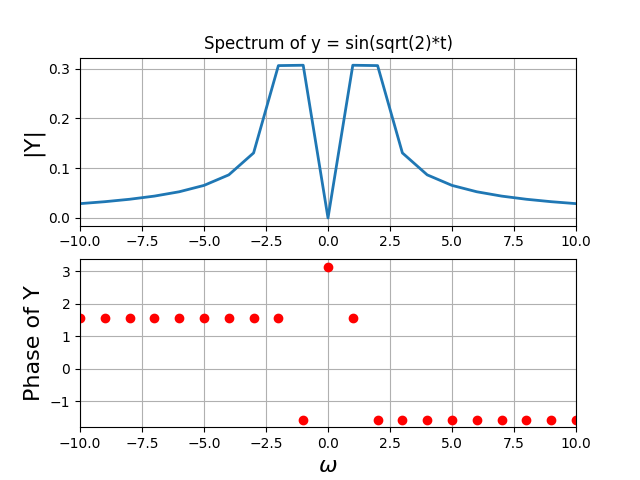
\includegraphics[scale=0.5]{A9_1.png} 
    \caption{DFT of $sin(\sqrt{2}t)$} 	
   \end{figure}   
   
   Instead of two spikes, we got two peaks. Figure 2 shows whats happening. The blue line connects the points whose DFT we took. The red lines show the continuation of the function. Quite clearly, even though $\sin(\sqrt{2} t)$ is a periodic function, the portion between $-\pi$ and $\pi$ is not the part that can be replicated to generate the function. The DFT is repeating the blue part which is not the periodic signal we started with. The reason is Gibbs phenomenon.

   
   \begin{figure}[!tbh]
   	\centering
  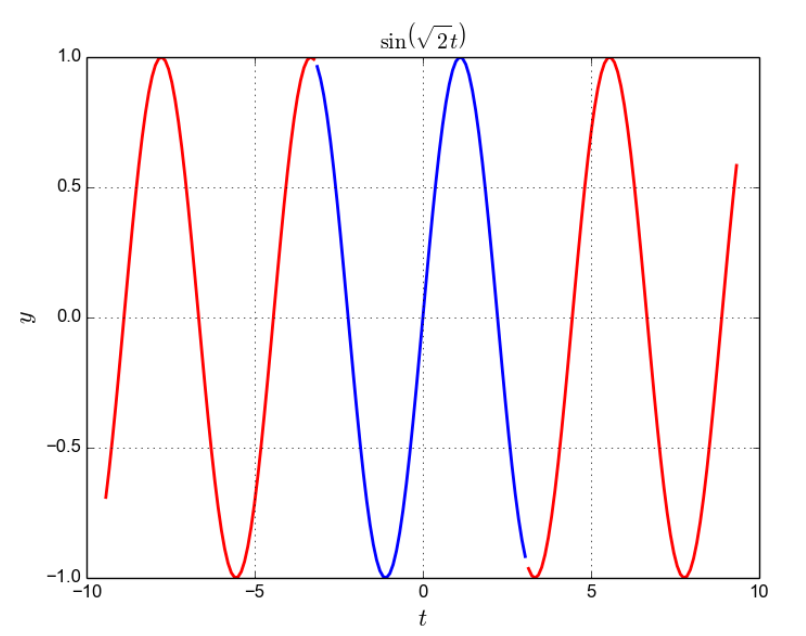
\includegraphics[scale=0.5]{q1.png} 
    \caption{tlim=4$\pi$, wlim=32, N=1024} 	
   \end{figure} 
   
     The DFT is just like the fourier series, except that both time and frequency are samples. So, if the time samples are like a ramp, the frequency samples will decay as $1/\omega$. So we use windowing. So we
damp the function near there, i.e., we multiply our function sequence f [n] by a “window” sequence w[n]: 
$$g(n)=f(n)w(n)$$
For a sinusoid, the two spikes will be smeared out by the window; so we expect to get broader peaks. This also suppresses the jump at the edge of the window. The Hamming Window:
$$w[n]=0.54+0.46\cos(\frac{2\pi n}{N-1})$$
for $|n|<=\frac{N-1}{2}$

This is what the sine looks like after windowing (Figure 3).  
\begin{figure}[!tbh]
   	\centering
  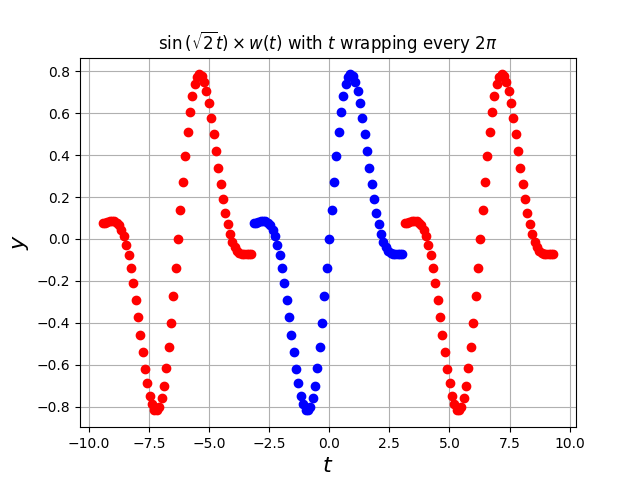
\includegraphics[scale=0.5]{A9_2.png} 
    \caption{$sin(\sqrt{2}t)*w(t)$ with t wrapping every $2\pi$} 	
   \end{figure}   

Now I execute the following code:
\begin{verbatim}
t = np.linspace(-np.pi, np.pi, 65)
t = t[:-1]
dt = t[1] - t[0]
fmax = 1 / dt
n = np.arange(64)
wnd = np.fft.fftshift(0.54 + 0.46 * 
np.cos(2 * np.pi * n / 63))
Y[0] = 0  # the sample corresponding to -tmax is 0
y = np.fft.fftshift(y)  # to make y start with 0
y = np.fft.fftshift(np.fft.fft(y)) / 64  # normalize
w = np.linspace(-np.pi * fmax, np.pi * fmax, 65)
w = w[:-1]
plt.figure()
plt.subplot(2, 1, 1)
plt.plot(w, abs(Y), lw=2)
plt.xlim([-8, 8])
plt.ylabel("|Y|", size=16)
plt.title("Spectrum of y = sin(sqrt(2)*t) with Hamming Window")
plt.grid()
plt.subplot(2, 1, 2)
plt.plot(w, np.angle(Y), "ro", lw=2)
plt.xlim([-8, 8])
plt.ylabel("Phase of Y", size=16)
plt.xlabel(r"$\omega$", size=16)
plt.grid()
plt.savefig("A9_3.png")
plt.show()

\end{verbatim}

\begin{figure}[!tbh]
   	\centering
  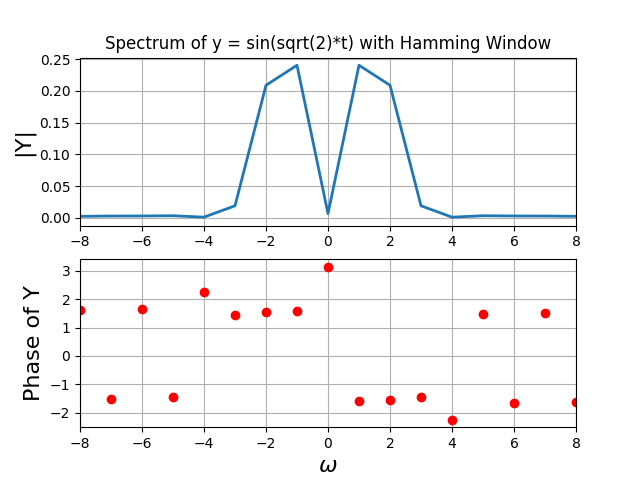
\includegraphics[scale=0.5]{A9_3.png} 
    \caption{$sin(\sqrt{2}t)*w(t)$ Spectra} 	
   \end{figure}  
   
\section{The Assignment}
\subsection{Question 2:} 
We need to plot the DFT of the function $\cos^3(0.86t)$
Without the Hamming Window
\begin{verbatim}
t = np.linspace(-np.pi, np.pi, 65)
t = t[:-1]
dt = t[1] - t[0]
fmax = 1 / dt
wo = 0.86
y = np.cos(wo * t) ** 3
y[0] = 0  # the sample corresponding to -tmax is 0
Y = np.fft.fftshift(y)  # to make y start with 0
Y = np.fft.fftshift(np.fft.fft(y)) / 64  # normalize
w = np.linspace(-np.pi * fmax, np.pi * fmax, 65)
w = w[:-1]
plt.figure()
plt.subplot(2, 1, 1)
plt.plot(w, abs(Y), lw=2)
plt.xlim([-10, 10])
plt.ylabel("Magnitude |Y|", size=16)
plt.title("Spectrum of y = cos^3(0.86t)")
plt.grid()
plt.subplot(2, 1, 2)
plt.plot(w, np.angle(Y), "ro", lw=2)
plt.xlim([-10, 10])
plt.ylabel("Phase of Y", size=16)
plt.xlabel(r"$\omega$", size=16)
plt.grid()
plt.savefig("A9_4.png")
plt.show()

\end{verbatim}

\begin{figure}[!tbh]
   	\centering
  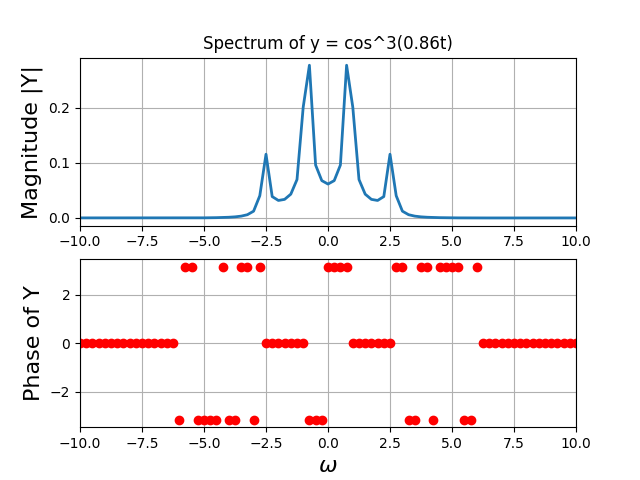
\includegraphics[scale=0.5]{A9_4.png} 
    \caption{$\cos^3(0.86t)$ DFT} 	
   \end{figure}  
   
With Hamming Window:
\begin{verbatim}
# with the Hamming Window
t = np.linspace(-np.pi, np.pi, 65)
t = t[:-1]
dt = t[1] - t[0]
fmax = 1 / dt
wo = 0.86
n = np.arange(64)
wnd = np.fft.fftshift(0.54 + 0.46 * 
np.cos(2 * np.pi * n / 63))
y = np.cos(wo * t) ** 3 * wnd
y[0] = 0  # the sample corresponding to -tmax is 0
Y = np.fft.fftshift(y)  # to make y start with 0
Y = np.fft.fftshift(np.fft.fft(y)) / 64  # normalize
w = np.linspace(-np.pi * fmax, np.pi * fmax, 65)
w = w[:-1]
plt.figure()
plt.subplot(2, 1, 1)
plt.plot(w, abs(Y), lw=2)
plt.xlim([-10, 10])
plt.ylabel("Magnitude |Y|", size=16)
plt.title("Spectrum of y = cos^3(0.86t) with Hamming Window")
plt.grid()
plt.subplot(2, 1, 2)
plt.plot(w, np.angle(Y), "ro", lw=2)
plt.xlim([-10, 10])
plt.ylabel("Phase of Y", size=16)
plt.xlabel(r"$\omega$", size=16)
plt.grid()
plt.savefig("A9_5.png")
plt.show()

\end{verbatim}
\begin{figure}[!tbh]
   	\centering
  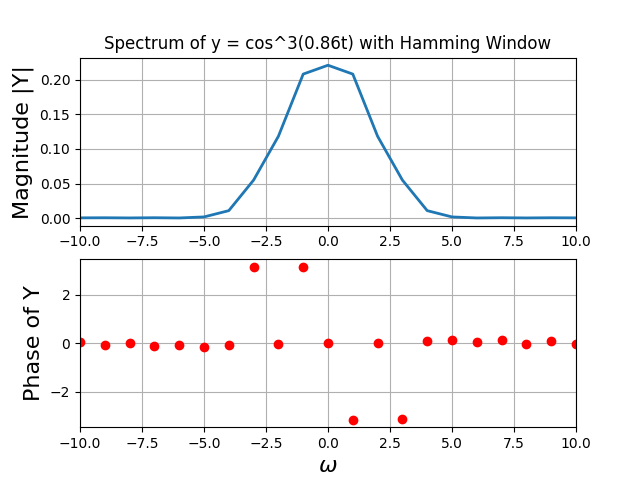
\includegraphics[scale=0.5]{A9_5.png} 
    \caption{$\cos^3(0.86t)$ DFT with Hamming Window} 	
   \end{figure}  
   
We see that the energy of the signal is distributed in many high frequencies that aren’t part of the actual signal, this energy gets attenuated after
performing windowing. 

\subsection{Question 3: Parameter Estimation}
We want to estimate $\omega$ and $\delta$ for the signal $\cos(\omega t+\delta)$, I have used a function \texttt{extract\_parameter} to find the unknowns from the given DFT array.

\begin{verbatim}
# Program to estimate frequency and phase of a signal
# cos(wo + d)
def extract_parameters(Y, w):
    # find the peak
    peak_index = np.argmax(abs(Y))
    # find the peak frequency
    peak_freq = w[peak_index]  # this is wo
    # now to find the phase
    phase = np.angle(Y[peak_index])
    return peak_freq, phase


# test the above function
x = np.linspace(0, 2 * np.pi, 129)
x = x[:-1]  # remove the last element
y = np.cos(10 * x + np.pi * 0.3)
Y = np.fft.fftshift(np.fft.fft(y)) / 128
wo, d = extract_parameters(Y, np.linspace(-64, 63, 128))
print("The frequency is:", wo, "and the phase is:", d)
# negative because it came first in the array
\end{verbatim}  

The result is printed out. It is negative because it came first in the DFT array, for symmetric functions one can use an absolute value. 
\begin{verbatim}
The frequency is: -10.0 and the phase is:
 -0.9424777960769362
\end{verbatim}

\subsection{Question 4: White Gaussian Noise}
Similar to the previous question with added random noise. 
\begin{verbatim}
# White Gaussian Noise
# Generate white Gaussian noise
noise = 0.1 * np.random.randn(len(Y))
# add noise to the signal
Y_noise = Y + noise
wo_noise, d_noise = extract_parameters(Y_noise,
 np.linspace(-64, 63, 128))
print("(Noise added) The frequency is:",
 wo_noise, "and the phase is:", d_noise)

\end{verbatim}
 
 Output
\begin{verbatim}
(Noise added) The frequency is: -10.0 and the 
phase is: -0.7729801795776737
\end{verbatim}   

\subsection{Question 5: Chirp Signal}
A frequency modulated signal
$$f(t)=\cos(16t(1.5+\frac{t}{2\pi}))$$

\begin{verbatim}
# The Chirped Signal
t = np.linspace(-np.pi, np.pi, 1025)
t = t[:-1]
dt = t[1] - t[0]
fmax = 1 / dt
y = np.cos(16 * t * (1.5 + t / (2 * np.pi)))
Y = np.fft.fftshift(np.fft.fft(y)) / 1024
w = np.linspace(-np.pi * fmax, np.pi * fmax, 1025)
w = w[:-1]
plt.figure()
plt.subplot(2, 1, 1)
plt.plot(w, abs(Y), lw=2)
plt.ylabel("Magnitude |Y|", size=16)
plt.title("Spectrum of y = cos(16t*(1.5+t/2pi))")
plt.xlim([-60, 60])
plt.grid()
plt.subplot(2, 1, 2)
plt.plot(w, np.angle(Y), "ro", lw=2)
plt.ylabel("Phase of Y", size=16)
plt.xlabel(r"$\omega$", size=16)
plt.xlim([-60, 60])
plt.grid()
plt.savefig("A9_6.png")
plt.show()


\end{verbatim}

We see that a large frequency appears as Gibbs frequency.
\begin{figure}[!tbh]
   	\centering
  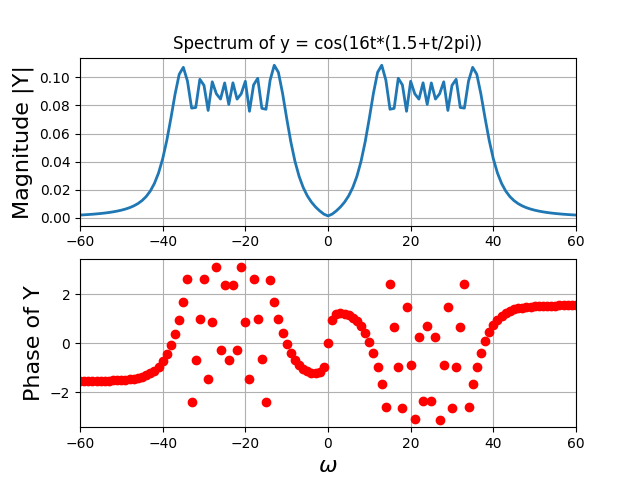
\includegraphics[scale=0.5]{A9_6.png} 
    \caption{Chirp Signal DFT} 	
   \end{figure}  
   
\subsection{Question 6}
For the same chirped signal, we break the 1024 vector into pieces that are 64 samples wide. Then plot the array as a surface plot to show how the frequency of the signal varies with time.

\begin{verbatim}
# Broken Chirped Signal; 16 parts
Y_array = []
for i in range(16):
    tlim1 = -np.pi + (2 * np.pi) * i / 16
    tlim2 = -np.pi + (2 * np.pi) * (i + 1) / 16
    t = np.linspace(tlim1, tlim2, 65)
    t = t[:-1]
    dt = t[1] - t[0]
    fmax = 1 / dt
    y = np.cos(16 * t * (1.5 + t / (2 * np.pi)))
    Y = np.fft.fftshift(np.fft.fft(y)) / 64
    Y_array.append((Y))

Y_array = np.array(Y_array)
t1 = np.linspace(-np.pi, np.pi, 16)
t = np.linspace(-np.pi, np.pi, 1025)
t = t[:-1]
dt = t[1] - t[0]
fmax = 1 / dt
w = np.linspace(-np.pi * fmax, np.pi * fmax, 65)
w = w[:-1]
t1, w = np.meshgrid(t1, w)
inds = np.where(abs(w) > 150)
Y_array[:, inds] = np.NaN
surface = axes3d.Axes3D(plt.figure())
s = surface.plot_surface(
    t1,
    w,
    abs(Y_array.T),
    rstride=1,
    cstride=1,
    cmap=cm.coolwarm,
    linewidth=0,
    antialiased=False,
)
plt.ylabel("Frequency", size=16)
plt.xlabel("Time", size=16)
plt.savefig("A9_7.png")
plt.show()

\end{verbatim}

\begin{figure}[!tbh]
   	\centering
  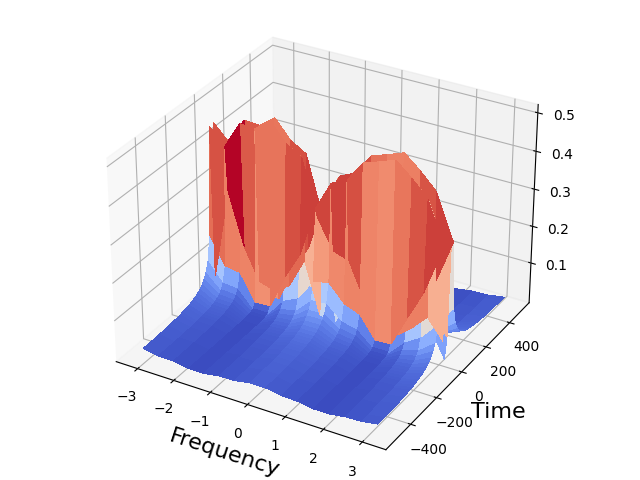
\includegraphics[scale=0.5]{A9_7.png} 
    \caption{Time Frequency Plot} 	
   \end{figure}  


\section{Conclusion}
The aim that we took at the beginning of this assignment is now seen to have been accomplished. I used of hamming window to find the DFT’s of aperodic signals. This was done to mitigate the effect of Gibbs phenomenon. The last question addresses the time varying spectra for a chirped signal, where I plotted Fourier spectra for different time slices of a signal.

\end{document}